%% ------------------------------------------------------------------------- %%
\chapter{A escolha do problema}
\label{cap:problema}

Na presente pesquisa demostraremos que o tipo de problema que gostaríamos de
resolver é: dado um conjunto armazenado em uma estrutura de acesso aleatório
aos seus índices (como um vetor) e uma operação associativa, desejamos responder 
eficientemente o resultado desta operação aplicada aos elementos de um intervalo 
desse conjunto múltiplas vezes.

\begin{figure}[htb]
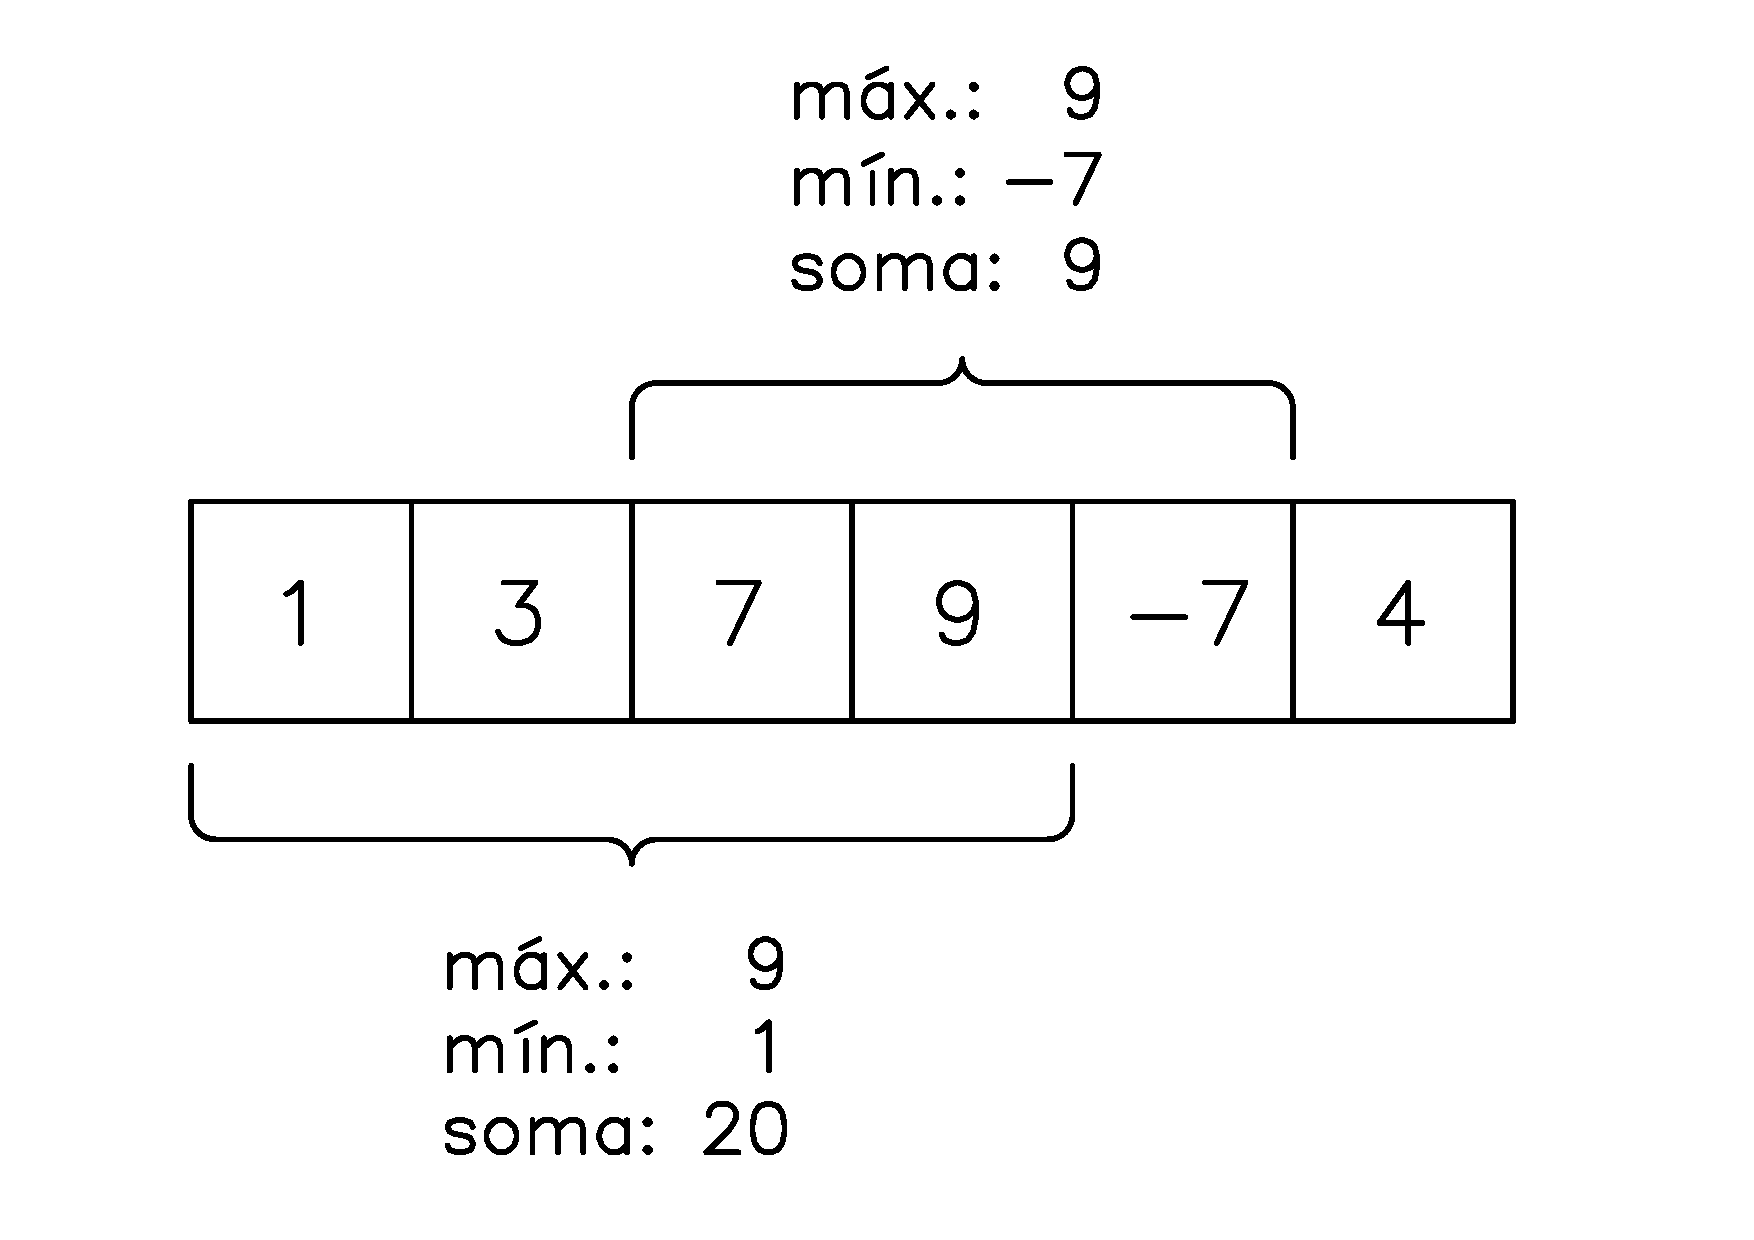
\includegraphics[width=12cm]{figuras/fig4.pdf}
\caption{\label{fig:fig4}Exemplo de estrutura, com operações aplicadas em intervalos.}
\end{figure}

\section{Motivação}
A motivação deste trabalho revela-se no fato de que problemas que envolvem 
realizar múltiplas consultas sobre o resultado de uma operação associativa em 
intervalos de um dado conjunto com relação de ordem nos índices, são encontrados 
em programação competitiva. Tendo em vista a robustez dos métodos utilizados para 
resolvê-los, esse tipo de problema aparece com uma frequência um pouco menor que 
outros problemas que envolvem algoritmos mais simples, razão pela qual dominar a 
solução deles trará o diferencial nas competições de programação.

\section{Objetivo}
O objetivo deste trabalho é tornar o estudo deste tópico menos penoso, uma vez 
que existe muito pouco material em língua portuguesa e que a maioria se limita a 
apontar uma implementação "caixa preta" pouco detalhada. Além disso, este material 
pretende servir como referência para todos que têm interesse em maratona de 
programação ou que gostariam de estudar e se aprofundar no tópico.

\section{Aplicação}
Seguindo com as possibilidades de aplicação do método, faz-se necessário 
aprofundarmos um pouco mais nos tipos de problemas tratados. Assim, considerando 
que dados n itens de supermercado; cada item possui um preço e um peso. Além 
disso, os n itens estão organizados por categoria, ou seja, primeiro os laticínios, 
depois os de limpeza, etc. Como administradores do supermercado, gostaríamos de 
todos os dias saber quais são os produtos mais baratos de cada categoria para que 
possamos preencher cartazes de promoção, levando em conta o fato de que todos os 
dias os preços de alguns dos produtos podem mudar.

Como clientes, temos acesso a listas de produtos como esta de vários supermercados 
e, com isso, gostaríamos de saber, naquele dia, em qual supermercado a soma de 
produtos de uma determinada categoria é menor, levando em conta promoções 
relâmpago.

Na ciência da computação a estrutura de dados que nos ajuda a resolver este tipo 
de problema é chamada de Árvore de Segmentos; tal estrutura é extremamente versátil,
baseada no paradigma de divisão e conquista, sendo possível idealizá-la como uma 
árvore usada para guardar informações sobre intervalos (segmentos) de um dado 
vetor (conjunto com relação de ordem nos índices) construída de tal forma a 
permitir perguntas e modificações a intervalos deste vetor de forma eficiente.

Uma das aplicações mais comuns desta estrutura envolve solucionar o problema 
do menor valor de um dado segmento, exemplificado acima pela lista de supermercado. 
Neste problema nos é dado um vetor com número e nos é perguntado inúmeras vezes 
qual é o menor valor de um dado intervalo.

\section{Exemplo}
Dado o seguinte vetor:

$$(1, 8, 2, 5, 4, 11, 3, 7)$$

Queremos saber o menor valor entre o terceiro e o quinto elemento: 
$min (2, 5, 4) = 2$

Depois gostaríamos de atualizar o valor do sexto elemento para 9, pois entramos 
em um período de promoção relâmpago para este produto, o que transforma o dado 
vetor em: 

$$(1, 8, 2, 5, 4, 9, 3, 7)$$

E agora perguntar qual o elemento mais barato entre o sexto e o oitavo: 
$min (9, 3, 7) = 3$

Divisão e conquista

A ideia da solução utilizando o paradigma de divisão e conquista conserva-se no 
seguinte raciocínio:

\begin{itemize}
    
    \item Se o intervalo que estamos analisando possui apenas um elemento então este 
elemento é trivialmente o menor do intervalo;

    \item Caso contrário, dividimos o intervalo em dois subintervalos de 
    aproximadamente mesmo tamanho, tomamos o mínimo de cada um deles e, como 
    a operação de mínimo é associativa, o mínimo deste intervalo é o mínimo 
    entre os dois mínimos sub intervalos;

\end{itemize}

Ou seja: 

\begin{center}
    $a_i$ se $x = y$ 
    \\
    ou
    \\
    $min (f(x, \lfloor{\frac{x+y}{2}}\rfloor)), f(\lfloor{\frac{x+y}{2}}\rfloor + 1, y)$ caso contrario.
\end{center}

Aplicações desta estrutura não se limitam a vetores de números inteiros e, 
frequentemente, são utilizados para resolver problemas em áreas como geometria 
computacional onde um ponto pode guardar muitas informações além de sua posição 
no plano.

\section{Observações}
Por outro lado, se tomarmos o já citado exemplo do supermercado e adicionarmos 
aos dados uma sacola com uma certa capacidade e perguntássemos qual é o 
subintervalo que cabe na sacola a considerar que a soma do peso de seus itens 
é menor ou igual a capacidade da sacola com a intensão de saber se isso maximiza 
a soma dos preços, infelizmente não seria possível encontrar a resposta através 
da utilização da árvore de segmentos, uma vez que a estrutura que aqui delineamos 
não resolve este problema diretamente.

Uma modificação simples que torna o problema bastante mais complexo, seria 
considerar um dado vetor de tamanho n e responder inúmeras vezes perguntas da 
seguinte natureza:

dado um intervalo e um número k, quantos elementos neste intervalo são maiores 
que k.

Imperioso salientar, ainda, que esta estrutura pode ser generalizada para mais 
do que uma dimensão.  

Neste sentido, veremos a seguir as formas de implementação da árvore de 
segmentos, entendendo melhor sua versatilidade e formas de aplicação.

